\documentclass[12pt]{article}
\usepackage[a4paper, hmargin=0.5in, vmargin=1in]{geometry}
\usepackage{microtype}
\usepackage{plex-otf}
% \usepackage{fontspec}
% \setmainfont{Times New Roman}

% \usepackage{csquotes}
\usepackage[bahasai]{babel}
% \usepackage{titling}
\usepackage{enumitem}
\usepackage{graphicx}
\usepackage{setspace}

% \usepackage[backend=biber, sorting=none, style=apa, refsection=section]{biblatex}
% \addbibresource{../../ref/library.bib}
\usepackage{hyperref}

\usepackage{lipsum}

\renewcommand{\baselinestretch}{1.5}
% \setlength{\parskip}{1em}

\usepackage{titlesec}
\titlelabel{\thetitle.\quad}
\titleformat*{\section}{\large\bfseries}

\newcommand{\mytitle}{UM162 - Pendidikan Pancasila}
\newcommand{\theauthor}{Rivo Juicer Wowor}
\newcommand{\affiliation}{00000059635}

\usepackage{fancyhdr}
\fancypagestyle{plain}{%
  \fancyhf{}%
  \lhead{\footnotesize{\textbf{\mytitle}}}%
  \fancyfoot[R]{\thepage}%
  \fancyfoot[L]{\footnotesize{\theauthor \hspace{1pt} (\affiliation)}}
}
 
\pagestyle{plain}

\begin{document}

\section{Proyek Kreatif Sosial Media Aksi Nyata Pancasila}
\begin{itemize}
    \item Produk kreatif yang kami buat adalah \textbf{situs web}.
    \item Situs web kami dapat diakses di tautan: \url{https://itshiroto.com/pkp-pancasila/}
    \item Selain itu, kami juga mengunggah poster di laman \emph{Instagram} kami 
          masing-masing:
        \begin{itemize}
          \item Rivo Juicer Wowor: \url{https://www.instagram.com/p/CW7yll2hFyw/}
          \item Fadhil Dzaky Muhammad: \url{https://www.instagram.com/p/CW7qtN3PeTt/}
          \item Resnu Wilmar: 
          \item Muhammad Farhan Efendi: \url{https://www.instagram.com/p/CW8FjG4lXlO/}
        \end{itemize}
\end{itemize}

\begin{minipage}[b]{0.47\textwidth}
    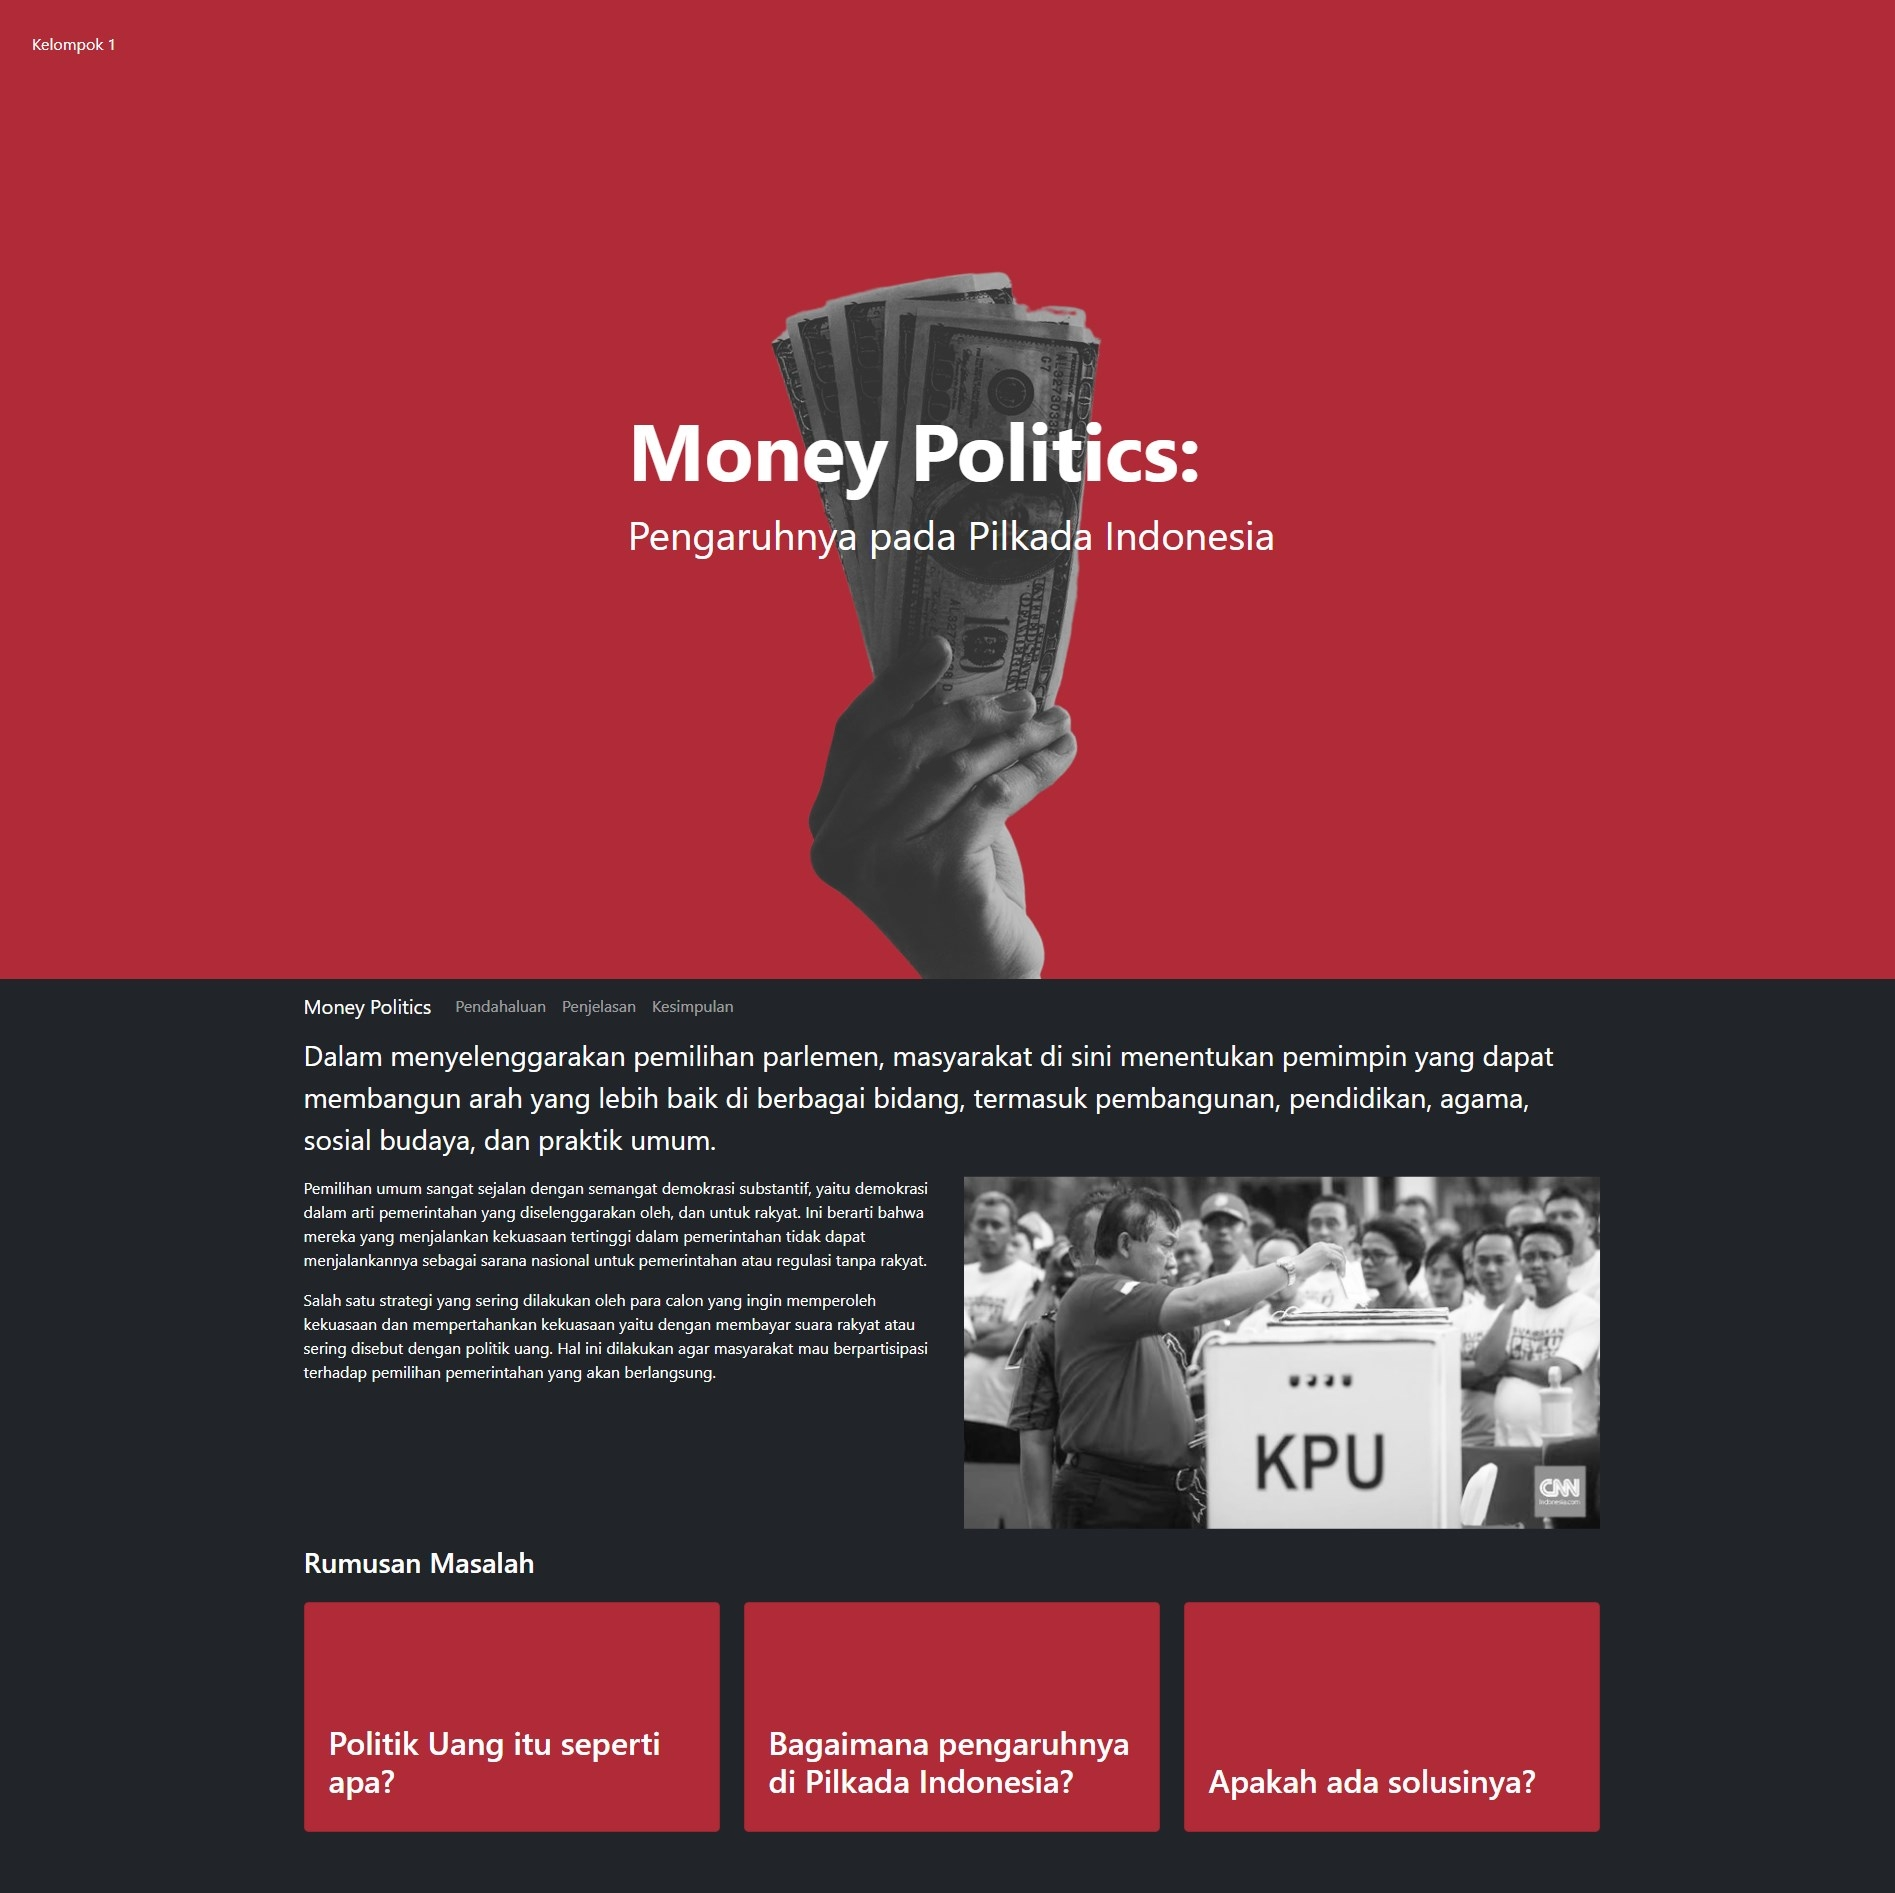
\includegraphics[width=\textwidth,keepaspectratio]{Asset/website.jpg}
\end{minipage}
\begin{minipage}[b]{0.47\textwidth}
    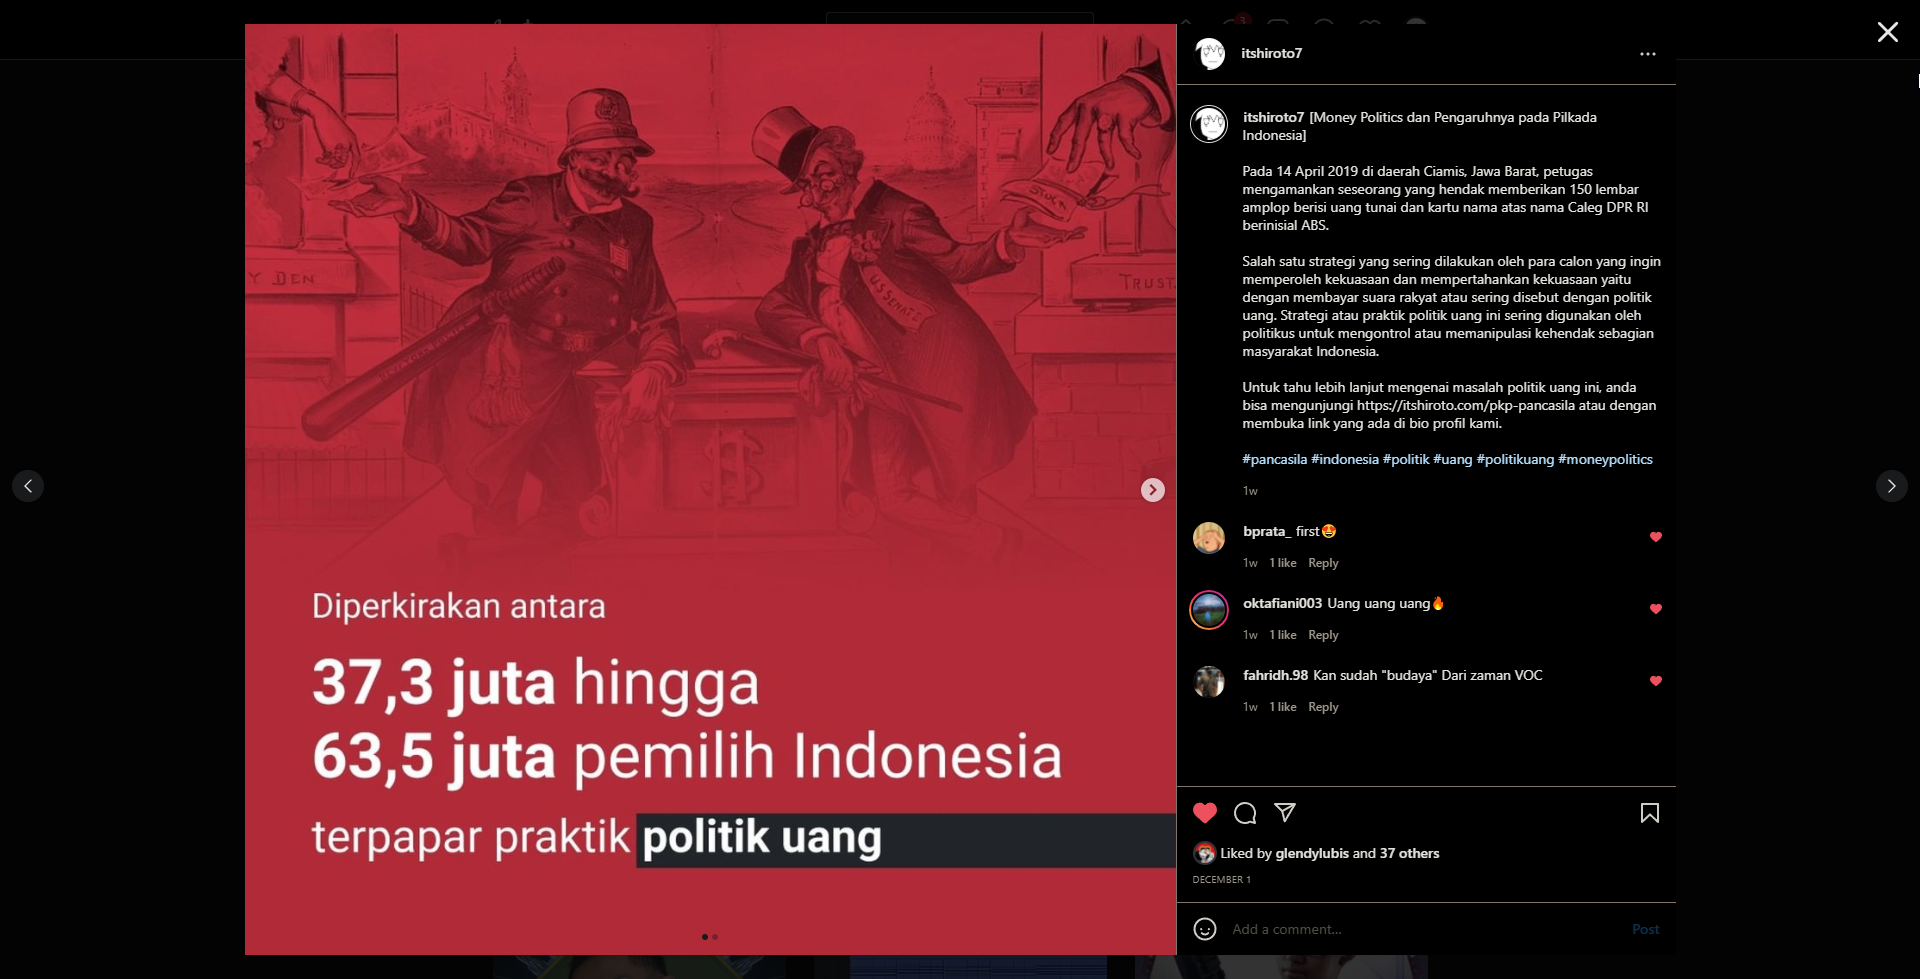
\includegraphics[width=\textwidth,keepaspectratio]{Asset/rivo.png}
    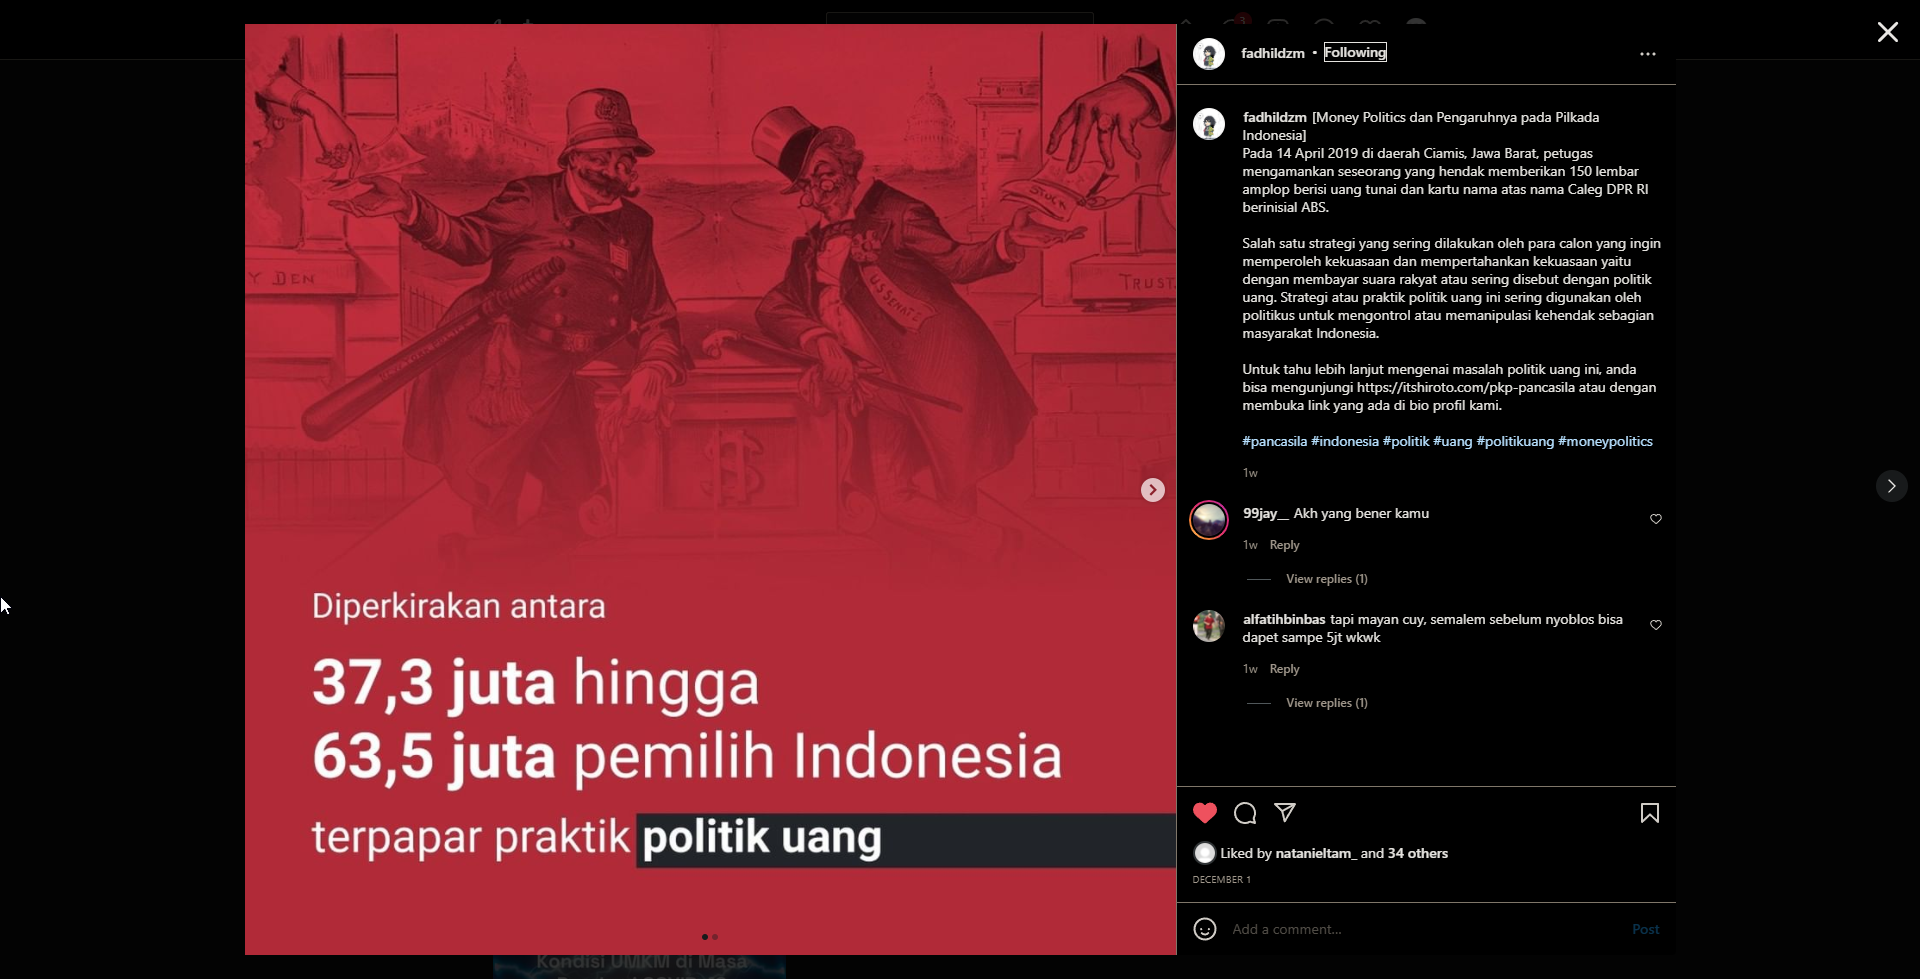
\includegraphics[width=\textwidth,keepaspectratio]{Asset/jaki.png}
    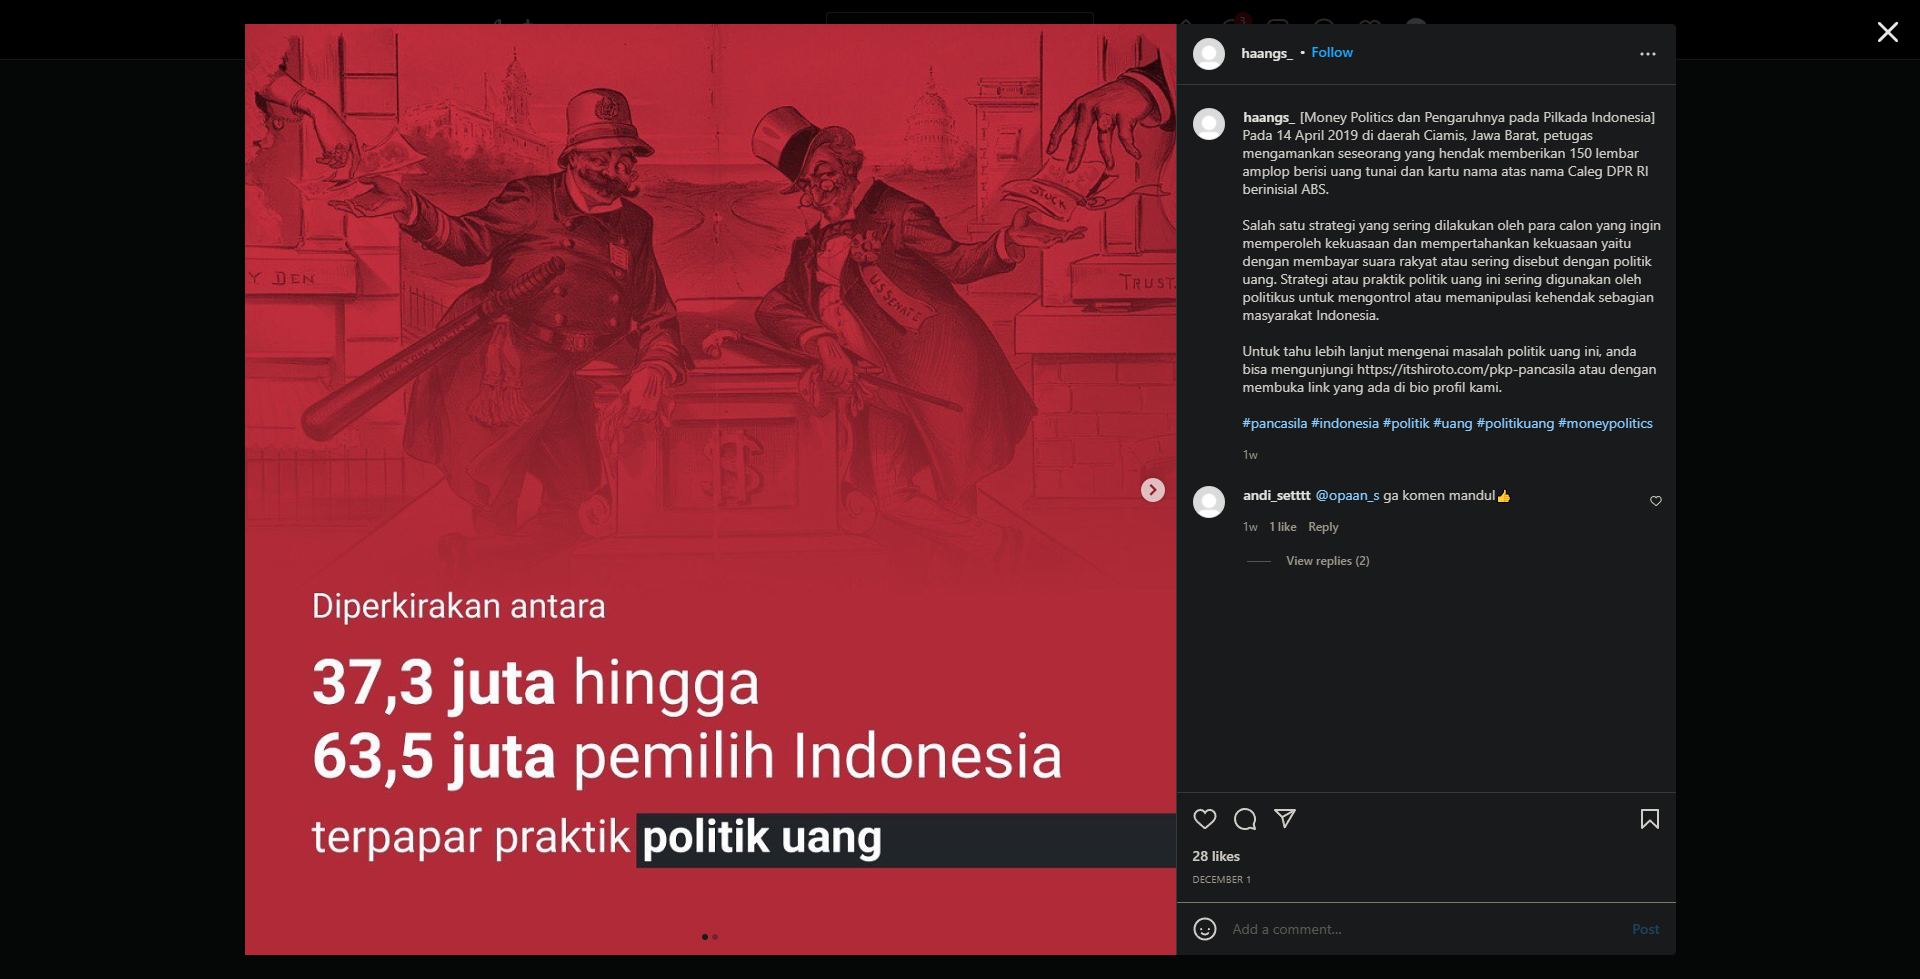
\includegraphics[width=\textwidth,keepaspectratio]{Asset/farhan.png}
    % 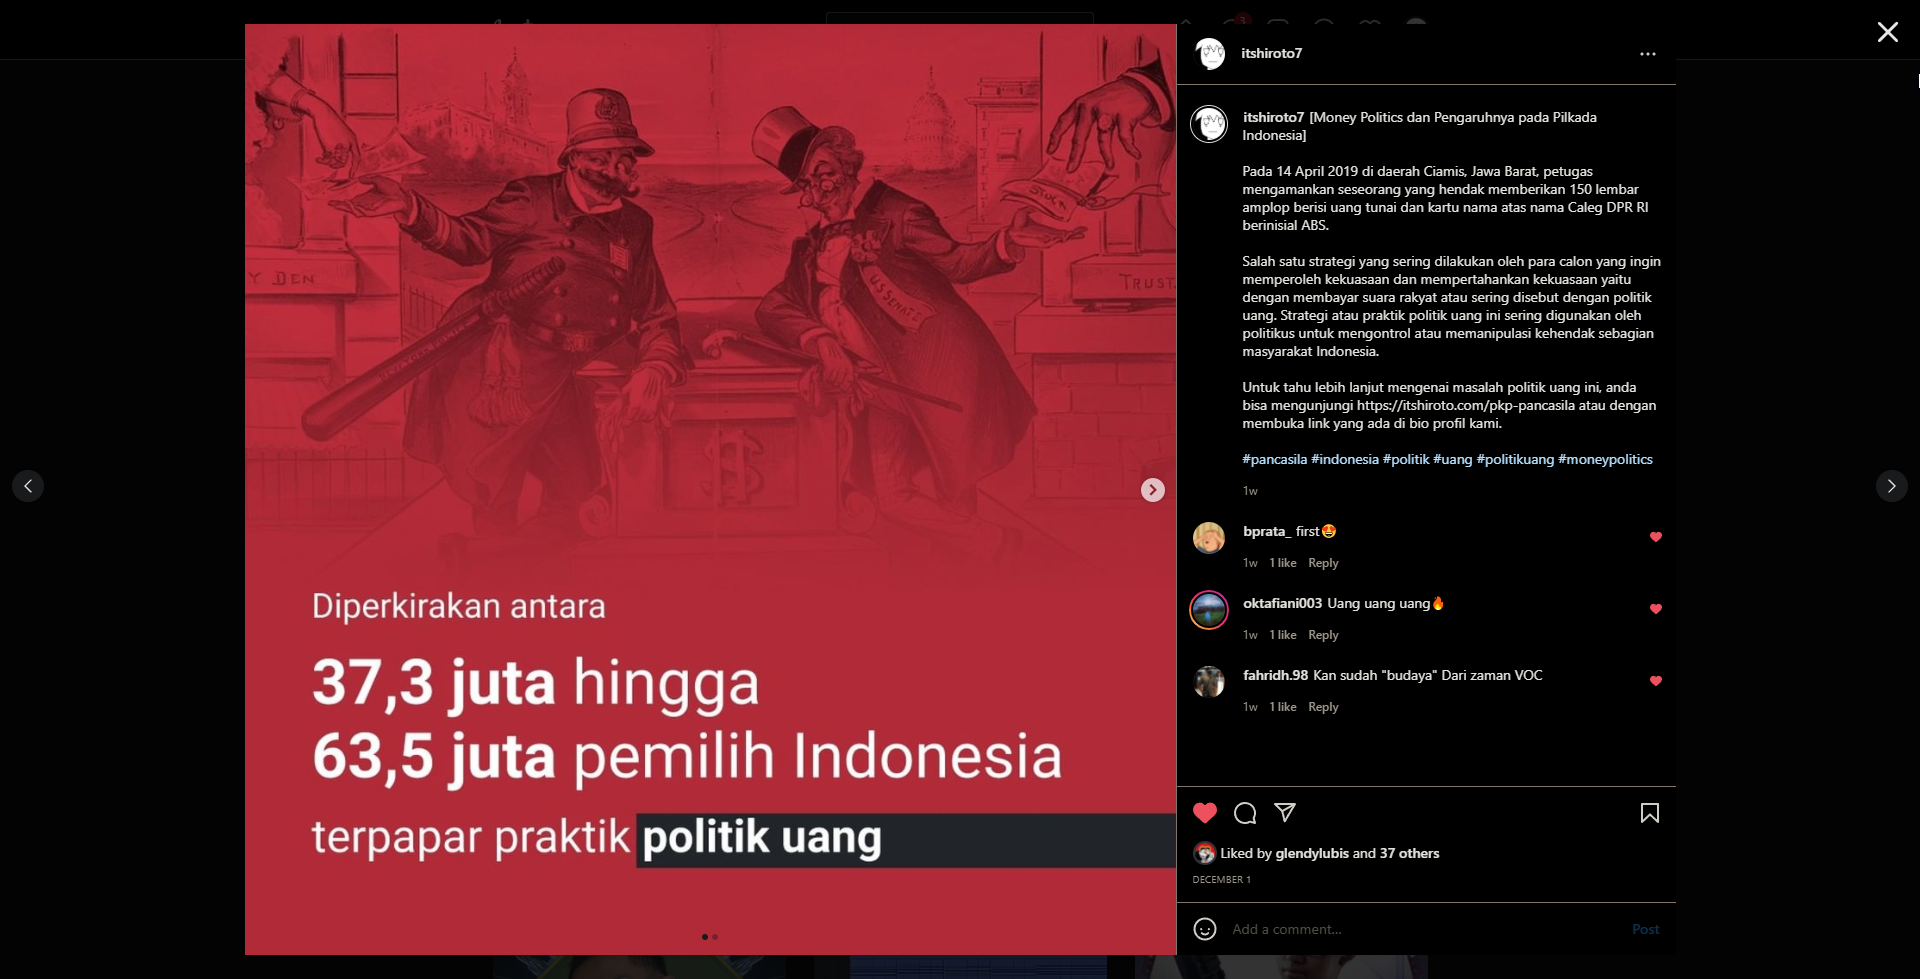
\includegraphics[width=\textwidth,keepaspectratio]{Asset/rivo.png}
\end{minipage}

\pagebreak

\section{Gotong Royong dan Aksi Nyata Pancasila}
\begin{enumerate}[label=\alph*)]
  \item
    Karena dalam pidatonya, Soekarno menegaskan bahwa Bangsa Indonesia 
    didirikan oleh orang-orang dengan berbagai latar belakang suku, agama, ras,
    dan golongan. Sehingga Soekarno mengusulkan bahwa Pancasila dapat diperas 
    menjadi suatu ekasila; yaitu Gotong Royong. Ia menjelaskan bahwa
    Gotong royong menggambarkan suatu usaha atau pekerjaan yang dilakukan secara
    bersama-sama oleh banyak orang. Hal gotong royong ini yang kami implementasikan
    ke dalam  proses pengerjaan proses kreatif kami, dimana kami membagi menjadi dua tim,
    yaitu \emph{developing} atau membuat situs web serta \emph{researching} atau
    mencari materi. meskipun memiliki tugasnya masing-masing tapi kami
    tetap bersama-sama membangun proyek kami yang berupa situs web ini secara
    bersama-sama.
  \item
    Menurut saya, kepedulian sosial merupakan suatu sikap dimana seorang
    manusia memiliki hubungan empati kepada sesamanya. Tentunya sikap ini
    sangat berkaitan dengan gotong royong karena gotong royong sendiri
    merupakan perwujudan bentuk kepedulian kita terhadap masyarakat
    untuk mencapai suatu tujuan. Dalam proses pengerjaan proyek kreatif juga,
    kami diajarkan juga secara tidak langsung bagaimana untuk bisa peduli
    terhadap teman sekelompok serta bekerja sama atau bergotong royong untuk
    bisa menyelesaikan proyek tersebut, dan juga belajar bagaimana membantu
    teman dan orang lain ketika mereka mengalami kesulitan dan masalah.
\end{enumerate}

\pagebreak

\section{Karakter dan Nilai-Nilai 5C}
\begin{enumerate}[label=\alph*)]
  \item
     Saya merasakan ada perubahan yang cukup signifikan dalam diri saya. Yaitu
     saya mulai belajar bagaimana caranya untuk berpikir secara kritis dan
     menggunakan akal sehat. Selain itu dengan mata kuliah Pancasila, saya
     menjadi lebih menghargai toleransi dan keberagaman yang ada di Indonesia;
     sesuai dengan semangat Pancasila yang dimiliki oleh Soekarno. Dan melalui
     proyek kreatifnya, saya juga belajar bagaimana berkomunikasi serta bekerja
     dengan sesama anggota kelompok saya.

  \item 
    Nilai 5C UMN juga merupakan salah satu faktor penting dalam perubahan yang
    saya alami ini. Ketika saya belajar bagaimana cara berpikir kritis, Nilai 
    \emph{Competent} yang menjadi salah satu alat pembantu saya untuk mengembangkan
    akal budi serta diri saya. Lalu nilai \emph{Caring} juga menjadi salah satu
    dampak besar ketika saya belajar bagaimana menghargai satu dengan yang lain.
    Lalu ada nilai \emph{Competitive}, \emph{Credible}, serta \emph{Customer Delight}
    juga membantu saya dalam bekerja secara kelompok dan juga menyampaikan
    presentasi di depan orang banyak.
\end{enumerate}

\section*{Pernyataan Pakta Integritas}
Segala hal yang saya nyatakan adalah benar

\vspace{3cm}

\singlespacing\noindent\begin{tabular}{l}
\makebox[2.5in]{\hrulefill} 
\vspace{0.5em} \\
Rivo Juicer Wowor \\
(00000059635)
\end{tabular}

\end{document}